%===================================== CHAP 8 =================================

\chapter{Evaluation}
\label{evaluationProcess}
This chapter contains evaluation of the process. Including the methodology, development and challenges the group have encountered.

\section{Methodology}
\label{evaluationMethodology}
During the project the group utilized scrum with sprints, consisting of stand-up- and daily meetings, in addition to sprint planning, -reviews and -retrospectives. This worked well, and led to all group members being aware of which issues the others were working on. 

Sprints was conducted with two weeks duration, which worked well for the group and the defined milestones. Sprint 2 was the only sprint the group did not manage to complete all issues in the backlog. The group encountered problems concerning technology in addition to under-estimations of tasks. Holding group meetings during the sprints was found good, essentially to help the scrum master and the other group members to be updated, and to prioritize the work remaining during each sprint. 

Using Waffle.io as a scrum-board worked great for the group. Getting a visualization of the progress of the project, specifically the milestones, was substantial for the planning throughout the project. The customer also had full access to the Waffle panel, were he could easily follow the project's progress, and add new milestones and issues to the project.

Based on the Extreme Programming principles, the group used pair programming. This was effective, as the pairs learned from each other as well as more than one member were aware of the status of each feature. Pair programming also gave the group validation when developing. Because there was always someone that reviewed the code, both logic and syntax.

\subsection{Development}
The development was influenced by the process, the methodology and the customer. The group developed in an iterative manner, and aimed to have new features implemented to present to the customer every week. Two times a week the group updated the live server with a new release. This way of development worked well. It made it possible for the group to focus on few set of features while working, and finalizing them before they started working on new features. Some features were more time consuming than others, and some of the features demanded that the group had to acquire new knowledge. The group worked together five days a week during the development process, this was not considered as too challenging. When a member got stuck or less motivated at times, the rest of the team was committed to contribute to help the member proceed and overcome eventual challenges.

To keep track of the features that was to be developed, the group used GitHub and Git to maintain the code. Every feature was developed on separate branches, thereafter merged with the main developing branch when the feature was completed. This was done up to several times during each sprint. When a sprint was finished the master branch was updated, which updated the production server. The customer appreciated that the application was rapidly updated on the production server, because he could test it whenever he desired and give the group feedback throughout the entire project period. This was helpful for the group, as it helped to prioritize which feature to implemented next, in addition to fixing bugs that occurred.


\subsection{Challenges}
A challenge to group encountered early in the project was to plan when to meet to work collaboratively as a group. Thus, there were some difficulties to plan a group time table, so that meetings and workdays would not collide with other subjects. Disregarding this challenge while getting started, it worked surprisingly well to work in a group of six over this period of time. The group had minor discussions, which were all resolved in collaboration. No issues led to dissatisfaction within the group.

Considering the group had decided to utilize new frameworks, libraries, working- and testing methods, some issues did occur. The group had some previous experience with Python, Javasript, HTML5 and CSS, but little experience with Django, React and Redux. Since all of this was new, the group spent a lot of time learning how to use the tools productively and correctly. 

During sprint 2 the group had minor problems getting started with Flux. The group spent a lot time trying to set up a good working environment with Flux, but could not manage to do so. After research and consulting with more experienced developers in this field, it was decided to use Redux instead. There were some challenges getting started with this library as well, but after a short period of time, the application was running smoothly with Redux. 

With the customer and users, the group faced a problem concerning how to present the facilitation for users. The customer was worried about being disrespectful by using symbols and words which described for whom an activity was facilitated for. After the second workshop, the children emphasized they wanted standard symbols, which directly told them if the activity was suited for them or not.    


\section{Cooperation With the Customer}
The group and the customer cooperated closely from the very beginning of project, which was especially appreciated by the group. There were arranged meetings every week, and the customer was very engaged in the project throughout the process. The customer and the group arranged workshops and focus groups with users. These helped the group to define the requirements, and to define suggestions to milestones for further development. The result is a proof of concept that verifies the need for this type of web portal.

The only, fairly minor, challenge the group encountered with the customer was the scope of a requirement was extended, giving the group more work than expected and estimated for the upcoming week. These extensions were good ideas, and therefore got the highest priority. The group also worked to satisfy the customers wishes, and the group believes that the customer was satisfied with the final product.


\section{Group Collaboration}
Since the start of the project, the group have been motivated to work hard with this project and has striven to satisfy the customer as much as possible. All of the group members know each other, and have worked together in previous projects. The group collaborated well throughout this project, and there have not been any big problems concerning communication within the group. If any misunderstandings appeared within the group either about the product, development or the process, issues was discussed and quickly reached a solution. With regards to the development, the group collaborated very well. If any issues came up, non of the members hesitated to ask for help from others. In several cases the members of the group also took the advantage of pair-programming to learn from each other and to achieve the best possible result.

\section{Project Management}
This section contains the updates to the risk analysis and evaluation of the hours worked in the project. 
\subsection{Risk Analysis}
\label{updated_risk_analysis}

During the project the group did not experience many disagreements or reasons for updating the risk analysis. Nevertheless, there were a few things that led to some updates. The risks were \textit{Group member being absent} and \textit{Misunderstanding of task}. The two risks are listed in table \ref{updated_risk_analysis_table}, containing the likelihood, impact, importance, preventive action and remedial action. 

\begin{longtable}{@{\extracolsep{\fill}}
                |L{0.14\linewidth}
                |L{0.09\linewidth}
                |L{0.09\linewidth}
                |L{0.14\linewidth}
                |L{0.17\linewidth}
                |L{0.17\linewidth}|@{}}
\hline


\rowcolor{Gray}
\textbf{Description} & \textbf{Likelihood (1-9)} & \textbf{ Impact (1-9)} & \textbf{Importance {\footnotesize (Likelihood * Impact)}} & \textbf{Preventive Action}    & \textbf{Remedial Action} \\ \hline
Group member being absent & 9 & 4 & 36 & Plan, add to common calendar, don’t take on big tasks in period when you are gone & Work in advance and make up for lost time \\
\hline
Misunderstanding of task & 8 & 7 & 56 & Open and frequent dialog with customer, agile dialog. & Make compromises, overtime and make up for lost time. \\
\hline
\caption{Updated Risk Analysis}
\label{updated_risk_analysis_table}
\end{longtable}


\subsection{Hours Worked}

The group worked well during the project time, the regular meetings helped to obtain progress and to keep track of what each member worked on (see table \ref{Hours_Worked} and figure \ref{Hours_Worked_Burndown}). This lead to the group following the schedule and the group were able to have code freeze as planed the 7th of April, at the end of sprint 4, together with error correction in sprint 5. The hours were distributed (see figure \ref{Distributed_Time}) between these different tasks from the work breakdown structure. The tasks are development, architecture and environment, design, testing, planning, project management including meetings within the group, with customer and supervisor, and report.
 

\begin{longtable}{@{\extracolsep{\fill}}
                |L{0.20\linewidth}
                |L{0.25\linewidth}
                |L{0.25\linewidth}
                |L{0.20\linewidth}|@{}}
\hline

\rowcolor{Gray}
\textbf{Sprint} & \textbf{Expected Time to Use} & \textbf{Used Hours} & \textbf{Difference} \\ 
\hline
Sprint 0 & 136h 30min & 124h 15min & 11h 45min  \\
\hline
Sprint 1 & 273h & 267h 35min & -3h 35min \\
\hline
Sprint 2 & 273h & 282h 45min & -9h 45min  \\
\hline
Sprint 3 & 273h & 306h 15min & -33h 15min  \\
\hline
Sprint 4 & 270h & 266h 40min &  6h 20min \\
\hline
Sprint 5 & 273h & 215h 5min & 57h 55min  \\
\hline
Sprint 6 & 352h 30min & h min & h min  \\
\hline
\textbf{Total} & \textbf{1854h} & \textbf{} & \textbf{} \\
\hline
\caption{Hours Worked}
\label{Hours_Worked}
\end{longtable}

\begin{figure}[H]
    \centering
    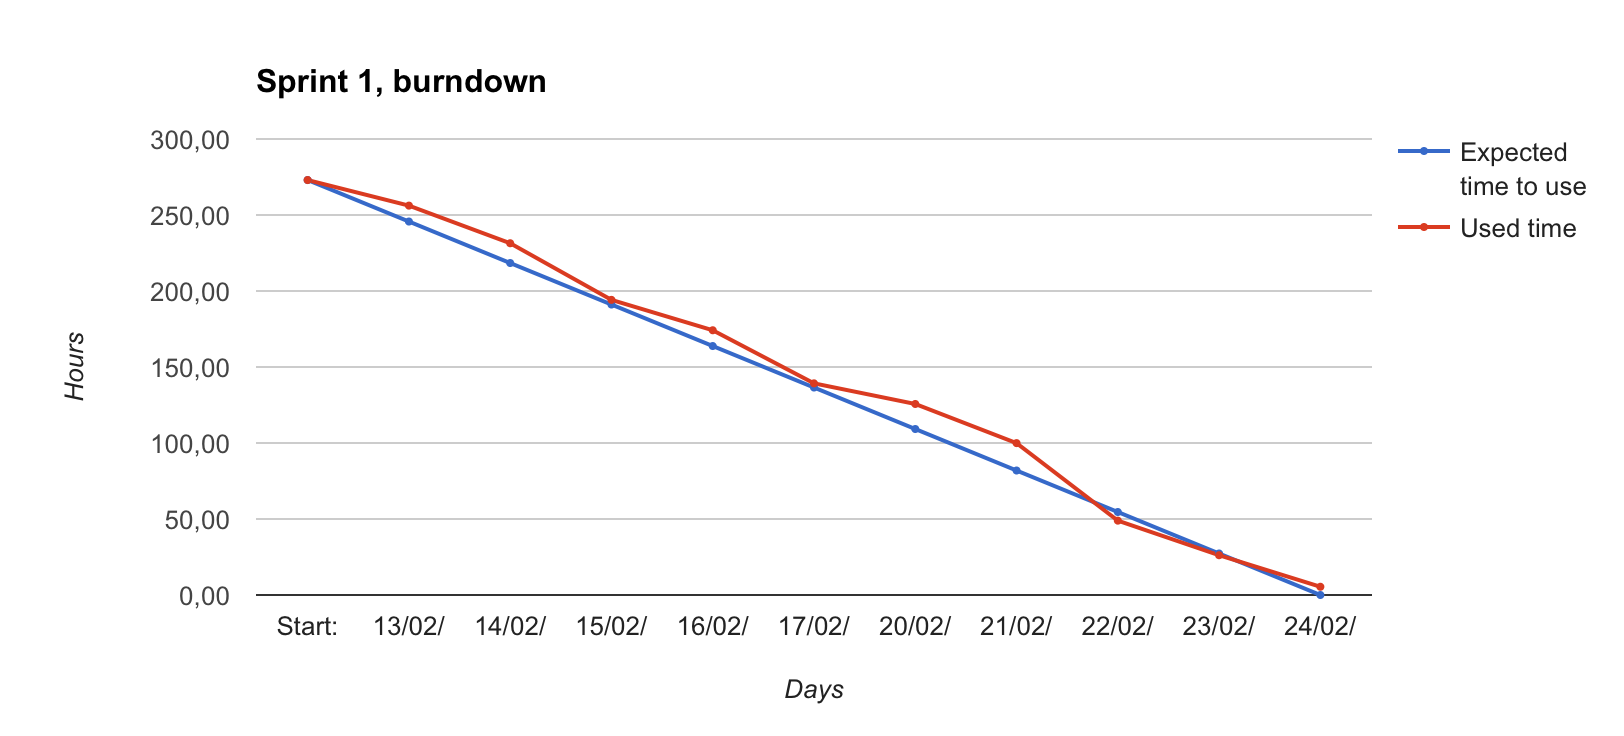
\includegraphics[width=\textwidth]{fig/sprint1}
    \caption{Sprint Burndown}
    \label{Hours_Worked_Burndown}
\end{figure}

\begin{figure}[H]
    \centering
    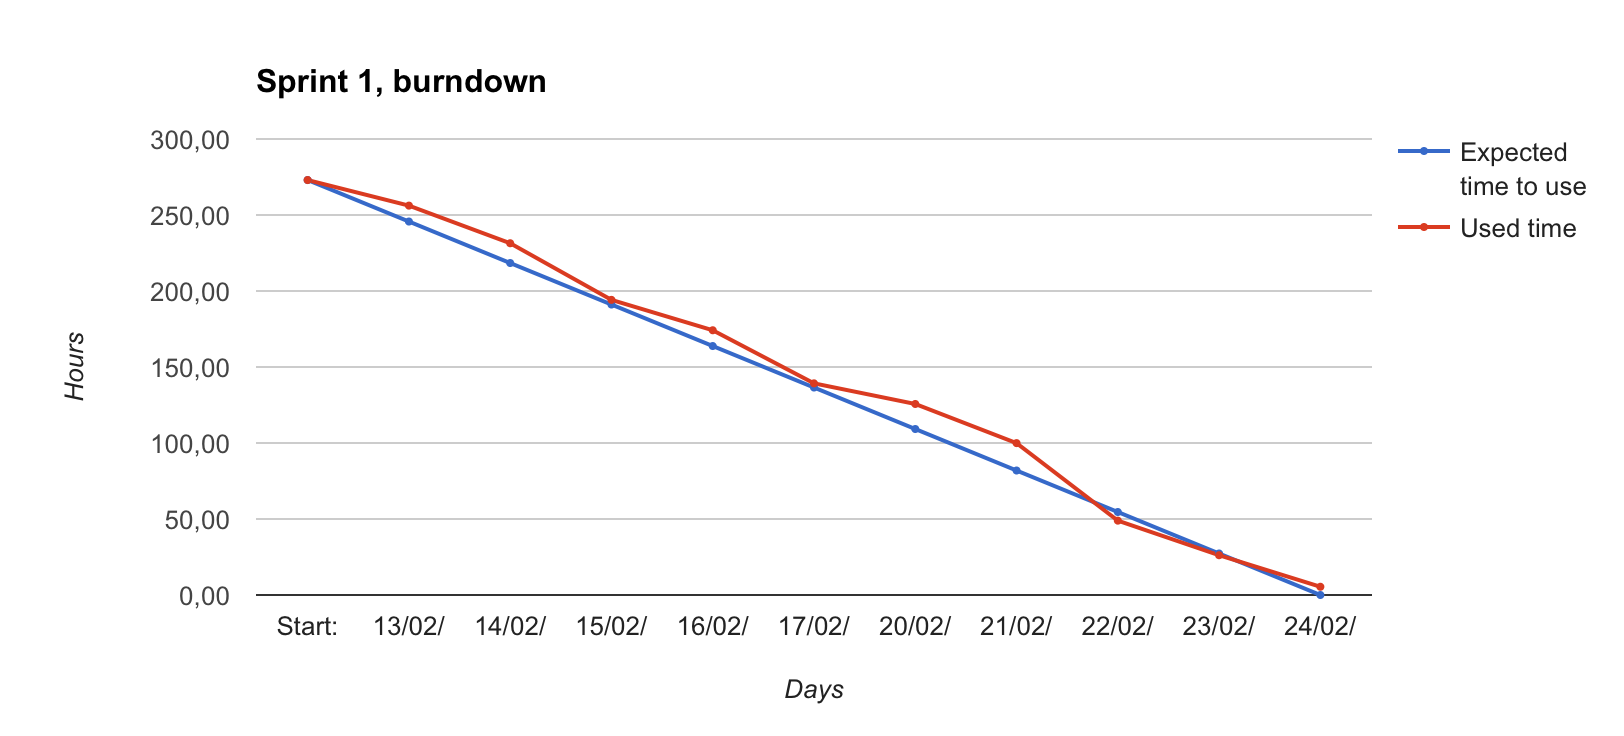
\includegraphics[width=\textwidth]{fig/sprint1}
    \caption{Distributed Time}
    \label{Distributed_Time}
\end{figure}

\section{Conclusion}
The workshop completed at the beginning of the project was used to gather as much information as possible, and to get a clear understanding of the users desired outcome of the project. The group organized all of the information so that it was possible to make use of it. During the project, the group actively used the customer to get feedback on the functionality implemented, and features desired to represent the concept. Together with the customer, group developed an application they believe suits the users. 

At the end of sprint 4 the group completed a focus group with providers to see what they thought about the web portal. The providers were happy with the result, and hoped that the development of the application would continue after the project was finished. In the beginning of sprint 5 the group had a new focus group with the families. This focus group turned out great. The families were satisfied with the portal and wished that the group could continue to work on it. 

The group are satisfied with the project, and have appreciated working with both the customer and different users. Throughout the entire project, the group has tried to satisfy both users and the customer, which it seems they have achieved. As a final conclusion the group would like to express the satisfaction of delivering a concept they are proud of, and a hope that the concept will be further developed to a final product in production.



\cleardoublepage